\documentclass{standalone}
\usepackage{tikz}
\usetikzlibrary{patterns, positioning}

\begin{document}
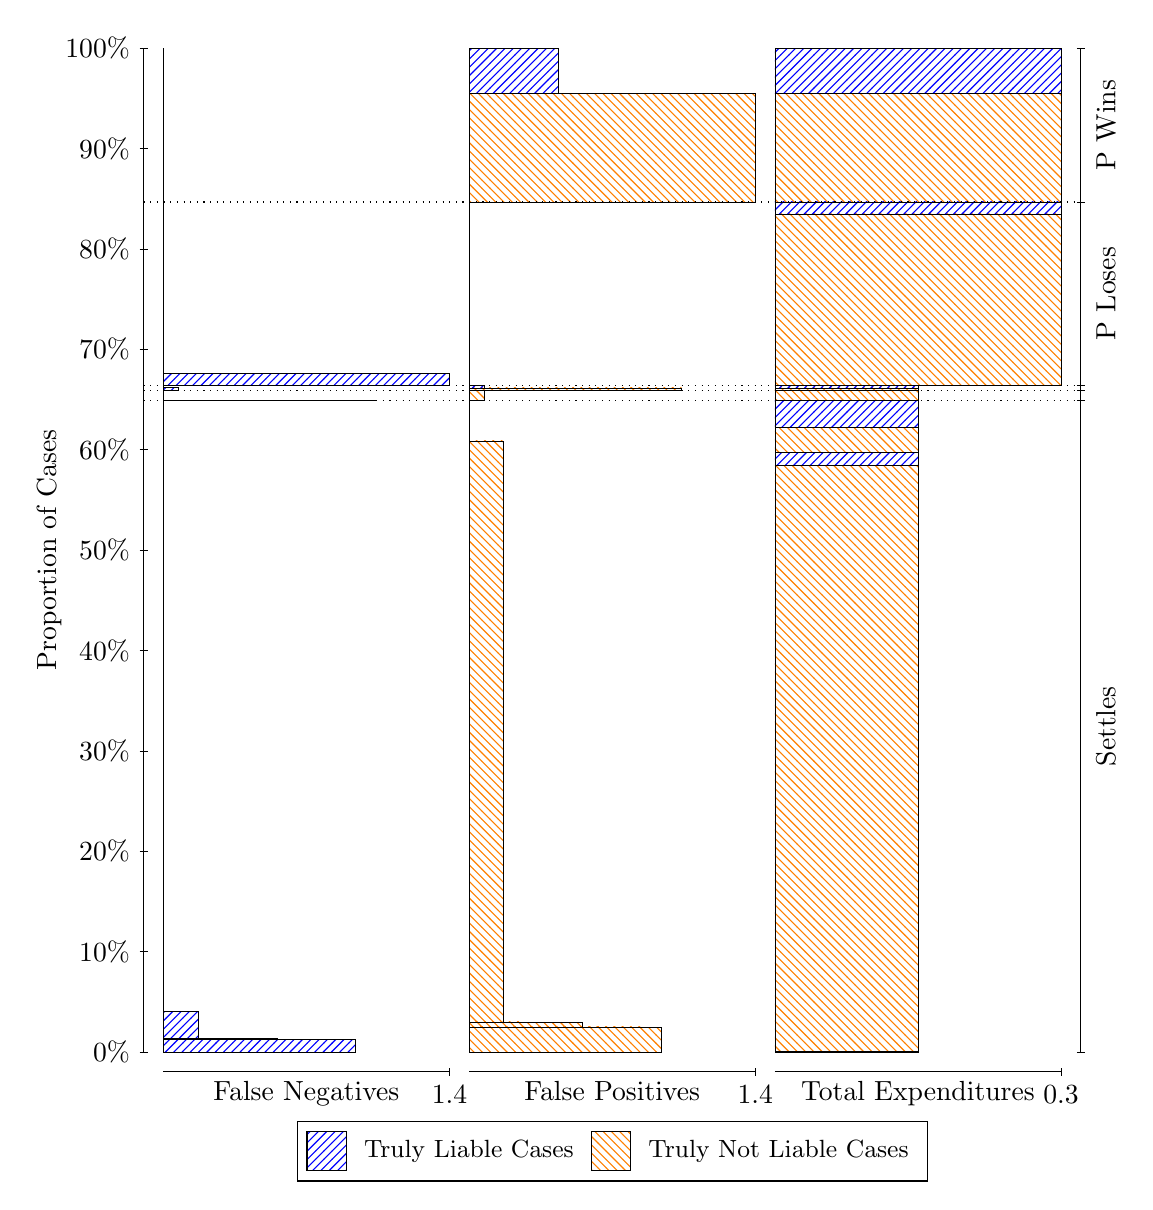
\begin{tikzpicture}
\draw[black, very thin] (1.5,1.75) -- (1.5,14.5);
\node[rotate=90, anchor=center] at (0.3, 8.125) {Proportion of Cases};
\draw[black, very thin] (1.45,1.75) -- (1.55,1.75);
\node[anchor=east] at (1.45, 1.75) {0\%};
\draw[black, very thin] (1.45,3.025) -- (1.55,3.025);
\node[anchor=east] at (1.45, 3.025) {10\%};
\draw[black, very thin] (1.45,4.3) -- (1.55,4.3);
\node[anchor=east] at (1.45, 4.3) {20\%};
\draw[black, very thin] (1.45,5.575) -- (1.55,5.575);
\node[anchor=east] at (1.45, 5.575) {30\%};
\draw[black, very thin] (1.45,6.85) -- (1.55,6.85);
\node[anchor=east] at (1.45, 6.85) {40\%};
\draw[black, very thin] (1.45,8.125) -- (1.55,8.125);
\node[anchor=east] at (1.45, 8.125) {50\%};
\draw[black, very thin] (1.45,9.4) -- (1.55,9.4);
\node[anchor=east] at (1.45, 9.4) {60\%};
\draw[black, very thin] (1.45,10.675) -- (1.55,10.675);
\node[anchor=east] at (1.45, 10.675) {70\%};
\draw[black, very thin] (1.45,11.95) -- (1.55,11.95);
\node[anchor=east] at (1.45, 11.95) {80\%};
\draw[black, very thin] (1.45,13.225) -- (1.55,13.225);
\node[anchor=east] at (1.45, 13.225) {90\%};
\draw[black, very thin] (1.45,14.5) -- (1.55,14.5);
\node[anchor=east] at (1.45, 14.5) {100\%};

\draw[black, very thin] (13.4,1.75) -- (13.4,14.5);
\draw[black, very thin] (13.35,1.75) -- (13.45,1.75);
\node[anchor=west] at (13.35, 1.75) {};
\draw[black, very thin] (13.35,10.023) -- (13.45,10.023);
\node[anchor=west] at (13.35, 10.023) {};
\draw[black, very thin] (13.35,10.152) -- (13.45,10.152);
\node[anchor=west] at (13.35, 10.152) {};
\draw[black, very thin] (13.35,10.218) -- (13.45,10.218);
\node[anchor=west] at (13.35, 10.218) {};
\draw[black, very thin] (13.35,12.545) -- (13.45,12.545);
\node[anchor=west] at (13.35, 12.545) {};
\draw[black, very thin] (13.35,14.5) -- (13.45,14.5);
\node[anchor=west] at (13.35, 14.5) {};

\draw[black, very thin, pattern color=blue, pattern=north east lines] (1.75,1.75) rectangle (4.1931,1.9071);
\draw[black, very thin, pattern color=blue, pattern=north east lines] (1.75,1.9071) rectangle (3.9425,1.9077);
\draw[black, very thin, pattern color=blue, pattern=north east lines] (1.75,1.9077) rectangle (3.692,1.9083);
\draw[black, very thin, pattern color=blue, pattern=north east lines] (1.75,1.9083) rectangle (3.4414,1.9089);
\draw[black, very thin, pattern color=blue, pattern=north east lines] (1.75,1.9089) rectangle (3.1908,1.9207);
\draw[black, very thin, pattern color=blue, pattern=north east lines] (1.75,1.9207) rectangle (2.9402,1.9208);
\draw[black, very thin, pattern color=blue, pattern=north east lines] (1.75,1.9208) rectangle (2.6897,1.9209);
\draw[black, very thin, pattern color=blue, pattern=north east lines] (1.75,1.9209) rectangle (2.4391,1.921);
\draw[black, very thin, pattern color=blue, pattern=north east lines] (1.75,1.921) rectangle (2.1885,2.2612);
\draw[black, very thin, pattern color=orange, pattern=north west lines] (1.75,2.2612) rectangle (1.75,10.023);
\draw[black, very thin, pattern color=blue, pattern=north east lines] (1.75,10.023) rectangle (4.4437,10.027);
\draw[black, very thin, pattern color=orange, pattern=north west lines] (1.75,10.027) rectangle (1.75,10.152);
\draw[black, very thin, pattern color=blue, pattern=north east lines] (1.75,10.152) rectangle (1.9379,10.186);
\draw[black, very thin, pattern color=orange, pattern=north west lines] (1.75,10.186) rectangle (1.75,10.218);
\draw[black, very thin, pattern color=blue, pattern=north east lines] (1.75,10.218) rectangle (5.3833,10.37);
\draw[black, very thin, pattern color=orange, pattern=north west lines] (1.75,10.37) rectangle (1.75,12.545);
\draw[black, very thin, pattern color=orange, pattern=north west lines] (1.75,12.545) rectangle (1.75,13.926);
\draw[black, very thin, pattern color=blue, pattern=north east lines] (1.75,13.926) rectangle (1.75,14.5);
\draw[black, very thin, pattern color=orange, pattern=north west lines] (5.6333,1.75) rectangle (8.0764,2.0669);
\draw[black, very thin, pattern color=orange, pattern=north west lines] (5.6333,2.0669) rectangle (7.8259,2.0673);
\draw[black, very thin, pattern color=orange, pattern=north west lines] (5.6333,2.0673) rectangle (7.5753,2.0676);
\draw[black, very thin, pattern color=orange, pattern=north west lines] (5.6333,2.0676) rectangle (7.3247,2.068);
\draw[black, very thin, pattern color=orange, pattern=north west lines] (5.6333,2.068) rectangle (7.0741,2.1228);
\draw[black, very thin, pattern color=orange, pattern=north west lines] (5.6333,2.1228) rectangle (6.8236,2.1229);
\draw[black, very thin, pattern color=orange, pattern=north west lines] (5.6333,2.1229) rectangle (6.8236,2.1258);
\draw[black, very thin, pattern color=orange, pattern=north west lines] (5.6333,2.1258) rectangle (6.573,2.1287);
\draw[black, very thin, pattern color=orange, pattern=north west lines] (5.6333,2.1287) rectangle (6.3224,2.1314);
\draw[black, very thin, pattern color=orange, pattern=north west lines] (5.6333,2.1314) rectangle (6.0718,9.5119);
\draw[black, very thin, pattern color=blue, pattern=north east lines] (5.6333,9.5119) rectangle (5.6333,10.023);
\draw[black, very thin, pattern color=orange, pattern=north west lines] (5.6333,10.023) rectangle (5.8213,10.148);
\draw[black, very thin, pattern color=blue, pattern=north east lines] (5.6333,10.148) rectangle (5.6333,10.152);
\draw[black, very thin, pattern color=orange, pattern=north west lines] (5.6333,10.152) rectangle (8.327,10.184);
\draw[black, very thin, pattern color=blue, pattern=north east lines] (5.6333,10.184) rectangle (5.8213,10.218);
\draw[black, very thin, pattern color=orange, pattern=north west lines] (5.6333,10.218) rectangle (5.6333,12.394);
\draw[black, very thin, pattern color=blue, pattern=north east lines] (5.6333,12.394) rectangle (5.6333,12.545);
\draw[black, very thin, pattern color=orange, pattern=north west lines] (5.6333,12.545) rectangle (9.2667,13.926);
\draw[black, very thin, pattern color=blue, pattern=north east lines] (5.6333,13.926) rectangle (6.7609,14.5);
\draw[black, very thin, pattern color=orange, pattern=north west lines] (9.5167,1.75) rectangle (11.333,1.7586);
\draw[black, very thin, pattern color=blue, pattern=north east lines] (9.5167,1.7586) rectangle (11.333,1.7604);
\draw[black, very thin, pattern color=orange, pattern=north west lines] (9.5167,1.7604) rectangle (11.333,9.1958);
\draw[black, very thin, pattern color=blue, pattern=north east lines] (9.5167,9.1958) rectangle (11.333,9.3646);
\draw[black, very thin, pattern color=orange, pattern=north west lines] (9.5167,9.3646) rectangle (11.333,9.6826);
\draw[black, very thin, pattern color=blue, pattern=north east lines] (9.5167,9.6826) rectangle (11.333,10.023);
\draw[black, very thin, pattern color=orange, pattern=north west lines] (9.5167,10.023) rectangle (11.333,10.148);
\draw[black, very thin, pattern color=blue, pattern=north east lines] (9.5167,10.148) rectangle (11.333,10.152);
\draw[black, very thin, pattern color=orange, pattern=north west lines] (9.5167,10.152) rectangle (11.333,10.184);
\draw[black, very thin, pattern color=blue, pattern=north east lines] (9.5167,10.184) rectangle (11.333,10.218);
\draw[black, very thin, pattern color=orange, pattern=north west lines] (9.5167,10.218) rectangle (13.15,12.394);
\draw[black, very thin, pattern color=blue, pattern=north east lines] (9.5167,12.394) rectangle (13.15,12.545);
\draw[black, very thin, pattern color=orange, pattern=north west lines] (9.5167,12.545) rectangle (13.15,13.926);
\draw[black, very thin, pattern color=blue, pattern=north east lines] (9.5167,13.926) rectangle (13.15,14.5);
\draw[black, dotted] (1.5,10.023) -- (13.4,10.023);
\draw[black, dotted] (1.5,10.152) -- (13.4,10.152);
\draw[black, dotted] (1.5,10.218) -- (13.4,10.218);
\draw[black, dotted] (1.5,12.545) -- (13.4,12.545);
\draw[black, very thin] (1.75,1.5) -- (5.3833,1.5);
\node[anchor=north] at (3.5667, 1.5) {False Negatives};
\draw[black, very thin] (5.3833,1.45) -- (5.3833,1.55);
\node[anchor=north] at (5.3833, 1.45) {1.4};

\draw[black, very thin] (5.6333,1.5) -- (9.2667,1.5);
\node[anchor=north] at (7.45, 1.5) {False Positives};
\draw[black, very thin] (9.2667,1.45) -- (9.2667,1.55);
\node[anchor=north] at (9.2667, 1.45) {1.4};

\draw[black, very thin] (9.5167,1.5) -- (13.15,1.5);
\node[anchor=north] at (11.333, 1.5) {Total Expenditures};
\draw[black, very thin] (13.15,1.45) -- (13.15,1.55);
\node[anchor=north] at (13.15, 1.45) {0.3};

\node[black, centered, rotate=90] at (13.72, 5.8866) {Settles};


\node[black, centered, rotate=90] at (13.72, 11.382) {P Loses};
\node[black, centered, rotate=90] at (13.72, 13.523) {P Wins};

\draw (7.449999999999999,1.5) node[draw=none] (baseCoordinate) {};
\begin{scope}[align=center]
        \matrix[scale=0.5, draw=black, below=0.5cm of baseCoordinate, nodes={draw}, column sep=0.1cm]{
            \node[rectangle, draw, minimum width=0.5cm, minimum height=0.5cm, pattern=north east lines, pattern color=blue] {}; &
            \node[draw=none, font=\small] (B) {Truly Liable Cases}; &
            \node[rectangle, draw, minimum width=0.5cm, minimum height=0.5cm, pattern=north west lines, pattern color=orange] {}; &
            \node[draw=none, font=\small] (B) {Truly Not Liable Cases}; \\
            };
\end{scope}

\end{tikzpicture}
\end{document}